\section{Evaluation}
\label{sec:evaluation}

We evaluate ParetoBandit across four experiments: stationary budget pacing, budget pacing under cost drift, resilience to silent quality degradation, and cold-start model onboarding. All experiments use 20~seeds and report 95\% bootstrap confidence intervals.

\subsection{Experimental Setup}
\label{sec:eval_setup}

\paragraph{Data and models.}
We collect 11,983 prompts from nine public NLP benchmarks (MMLU~\cite{hendrycks2021measuring}, GSM8K~\cite{cobbe2021gsm8k}, HellaSwag~\cite{zellers2019hellaswag}, BIG-Bench Hard~\cite{suzgun2022challenging}, ARC-Challenge~\cite{clark2018arc}, OpenBookQA~\cite{mihaylov2018suit}, WinoGrande~\cite{sakaguchi2020winogrande}, TruthfulQA~\cite{lin2022truthfulqa}, MBPP~\cite{austin2021program}) spanning reasoning, math, code synthesis, commonsense, and factual knowledge. For each prompt, all $K{=}3$ models generate responses that are judged offline, producing a full reward--cost matrix. Prompts are partitioned into three disjoint splits stratified by source: train ($n{=}8{,}374$) for fitting warmup priors, val ($n{=}1{,}785$) for online hyperparameter tuning, and test ($n{=}1{,}824$) for evaluation. The $K{=}3$ portfolio spans a $\bpPriceRangeX{\times}$ cost range (Table~\ref{tab:setup}).

\paragraph{Quality evaluation.}
Each response is scored by DeepSeek-R1~\cite{deepseekai2025deepseekr1} on three continuous dimensions: reasoning quality (weight 0.4), instruction following (0.3), and communication quality (0.3), yielding a composite reward $r_t \in [0, 1]$. R1 produces the largest inter-model reward gaps among the judges we evaluated; Appendix~\ref{sec:judge_robustness} validates that its routing decisions capture ${\geq}97\%$ of any alternative judge's oracle reward.

\paragraph{Baselines.}
Two conditions represent increasing routing sophistication, all sharing warmup priors ($n_\mathit{eff}{=}\bdNeff$, $\alpha{=}\ppAlpha$):
\begin{enumerate}[nosep,leftmargin=*]
  \item \textbf{Naive Bandit ($\gamma{=}1.0$):} LinUCB with online learning but infinite memory and a static cost penalty.
  \item \textbf{ParetoBandit ($\gamma{=}\ppGamma$):} Geometric forgetting with warmup priors and an active BudgetPacer.
\end{enumerate}
Experiment~2 additionally includes a \textbf{Recalibrated Bandit} (oracle knowledge of price changes) and a \textbf{Forgetting Bandit} ($\gamma{=}\ppGamma$, no pacer) as ablations. Hyperparameters are selected via the Pareto knee-point procedure described in Appendix~\ref{sec:hparam_sweep}.

\noindent\textbf{Non-stationary protocol.} Experiments 2--3 follow a three-phase stress-test: normal operation (608 prompts), abrupt perturbation (608 prompts), and recovery (608 prompts). Phase~3 reuses Phase~1 prompts for a controlled within-subject comparison.

\vspace{-6pt}
\begin{table}[!htbp]
\centering
\caption{Model portfolio and budget targets. The $\bpPriceRangeX{\times}$ cost spread stresses the router's quality--cost tradeoff. Three budgets span the full operating range.
}
\label{tab:setup}
\small
\begin{tabular}{@{}llr@{}}
\toprule
\textbf{Model} & \textbf{Tier} & \textbf{Cost (\$/req)} \\
\midrule
Llama-3.1-8B   & Budget   & $\$2.9{\times}10^{-5}$ \\
Mistral-Large  & Mid-cost & $\$5.3{\times}10^{-4}$ \\
Gemini-2.5-Pro & Frontier & $\$1.5{\times}10^{-2}$ \\
\midrule
\textbf{Budget} & \textbf{Target $B$} & \textbf{Regime} \\
\midrule
Tight    & $\$3.0{\times}10^{-4}$ & Llama-dominant \\
Moderate & $\$6.6{\times}10^{-4}$ & Llama--Mistral mix \\
Loose    & $\$1.9{\times}10^{-3}$ & Selective Gemini \\
\bottomrule
\end{tabular}
\end{table}

\subsection{Stationary Budget Pacing}
\label{sec:eval_stationary}

We first ask: \emph{can the router accept a dollar budget ceiling and automatically maximize quality beneath it, filling the quality--cost gaps between fixed single-model baselines?}

Figure~\ref{fig:pareto}a shows the quality--cost Pareto frontier on the test set. Each fixed model occupies a single point on this frontier, plotted as (mean cost per request, mean quality score): Llama at ($\bpFixedLlamaCost$, $\bpFixedLlamaReward$), Mistral at ($\bpFixedMistralCost$, $\bpFixedMistralReward$), Gemini at ($\bpFixedGeminiCost$, $\bpFixedGeminiReward$). The BudgetPacer traces a continuous curve through these points by dynamically mixing models based on prompt context and budget pressure. At a budget of $\bpAnnotBudget$/req, the router achieves $\bpAnnotQualPct$\%\,[$\bpAnnotQualPctCILo$, $\bpAnnotQualPctCIHi$] of Gemini quality at $\bpAnnotCostPct$\% of its cost by blending $\bpAnnotLlamaFrac$\% Llama and $\bpAnnotMistralFrac$\% Mistral. For binding ceilings, utilisation ranges from $\bpUtilBindingLow$ to $\bpUtilBindingHigh$ (Figure~\ref{fig:pareto}b). When the ceiling is high enough that cost never binds, the cost penalty $\lambda_t$ decays to zero and the router reduces to pure quality maximization, recovering $\bpCeilingOraclePct$\%\,[$\bpCeilingOraclePctCILo$, $\bpCeilingOraclePctCIHi$] of an oracle that selects the highest-scoring model for each prompt ($\bpOracleReward$). In practice, this turns model selection from a discrete choice among $K$ fixed operating points into a continuous budget dial: the operator sets a dollar ceiling, and the router discovers the best quality mix beneath it (Figure~\ref{fig:pareto}c).

\begin{figure*}[!t]
\centering
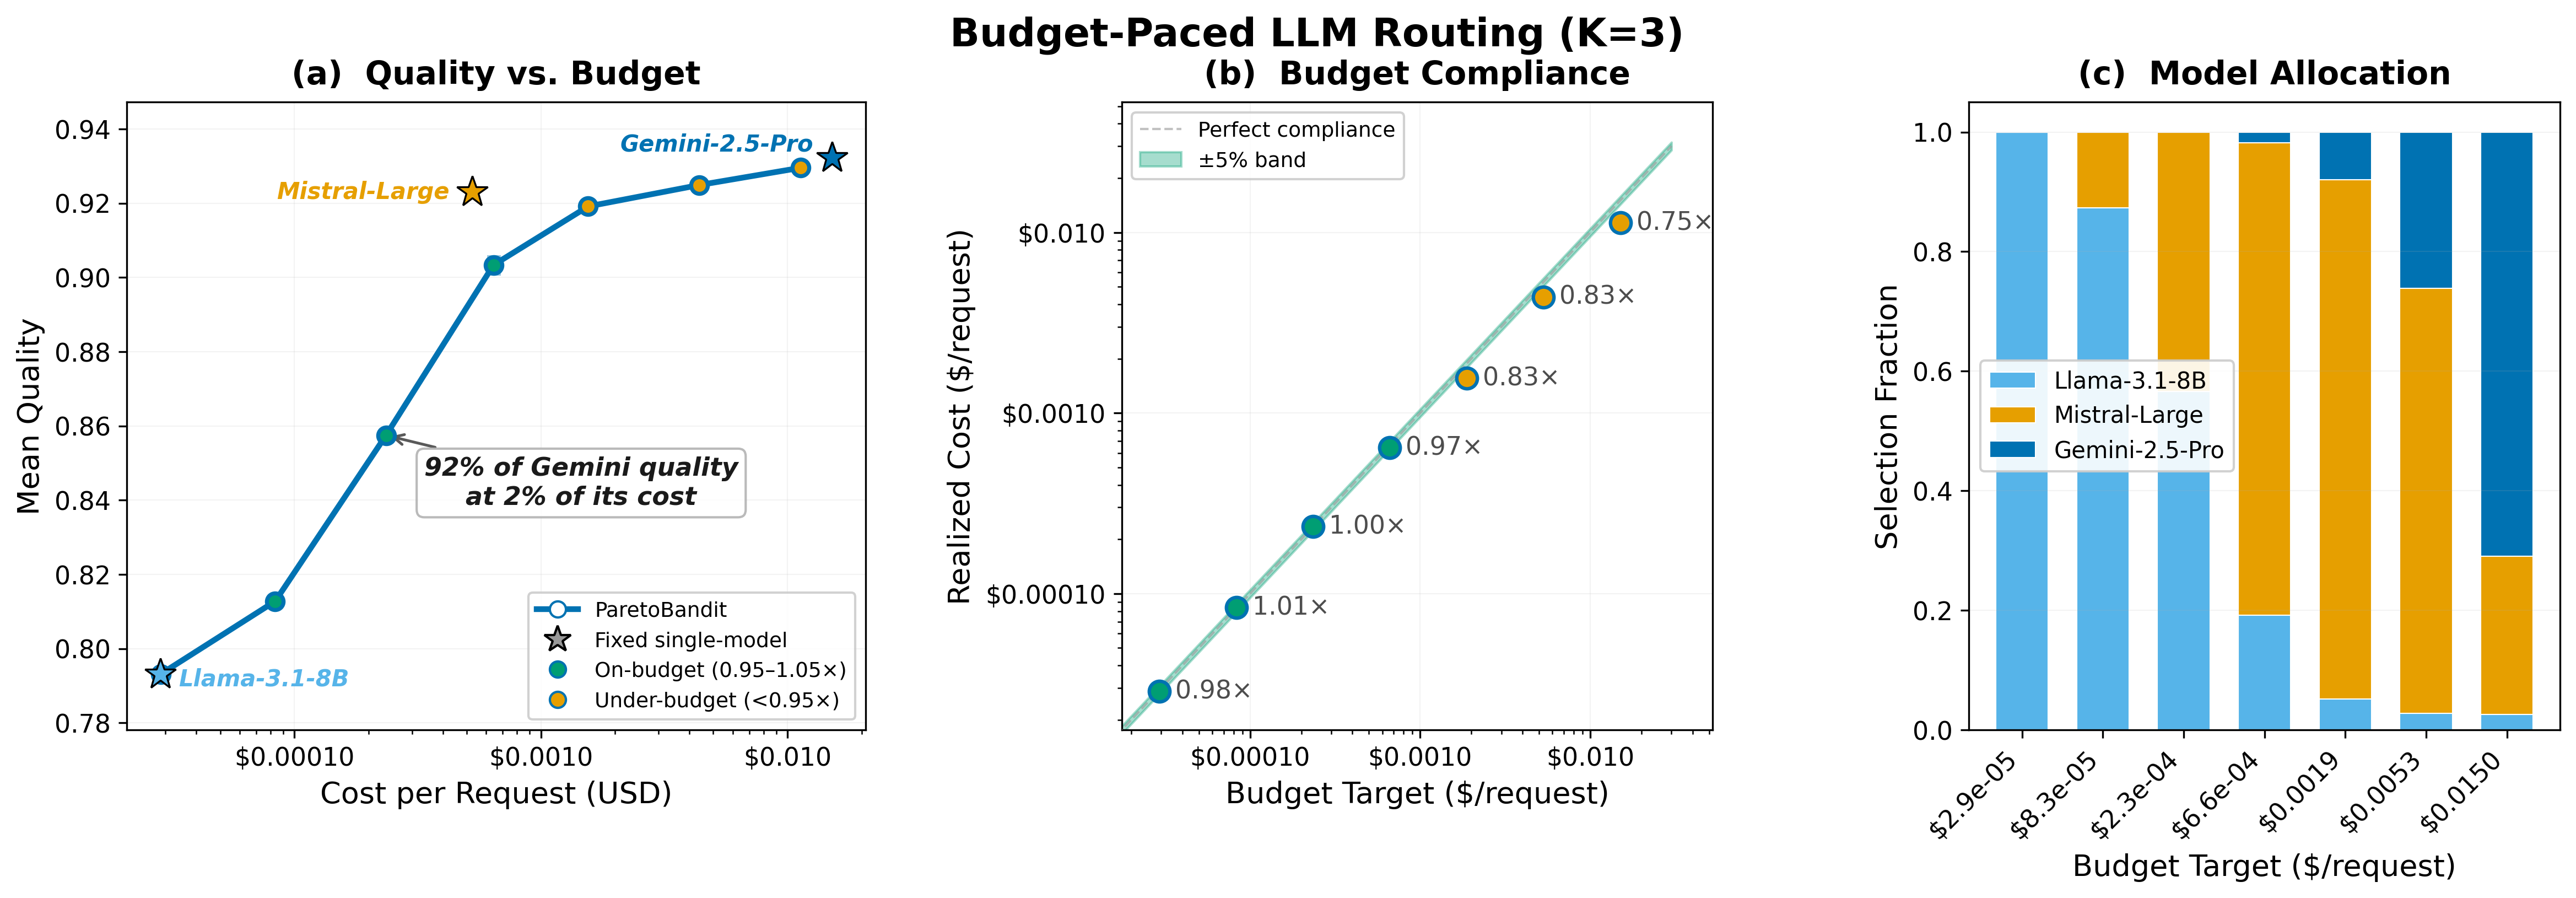
\includegraphics[width=\textwidth]{../experiments/01_stationary_budget_pacing/results/budget_pacing.png}
\caption{Quality--cost Pareto frontier under stationary conditions ($K{=}3$, 20~seeds). \textbf{(a)}~ParetoBandit with BudgetPacer (blue curve) traces a continuous quality--cost frontier by accepting a dollar budget ceiling. Fixed single-model baselines shown as stars. \textbf{(b)}~Budget compliance: realized cost vs.\ ceiling. Green band marks $\pm5\%$. \textbf{(c)}~Model allocation shifts from Llama-dominant at tight budgets to Gemini-heavy at loose budgets.
}
\label{fig:pareto}
\vspace{4pt}
\end{figure*}

\subsection{Budget Pacing under Cost Drift}
\label{sec:eval_nonstationary}

We now evaluate whether the pacer automatically exploits a mid-stream price drop while maintaining compliance. Phase~1 uses normal pricing; Phase~2 drops Gemini-2.5-Pro's pricing to \$0.10/M tokens (normalized cost $\tilde{c} \approx 0$); Phase~3 restores original pricing.

\noindent\textbf{Budget compliance is the key differentiator.}
Table~\ref{tab:budget_compliance} summarises cost/ceiling ratios across all conditions and phases. ParetoBandit is the only condition that reliably stays within the ceiling in Phase~1 ($\bdParetoBanditLoosePhaseOneRatio$\,[$\bdParetoBanditLoosePhaseOneRatioCILo$, $\bdParetoBanditLoosePhaseOneRatioCIHi$] to $\bdParetoBanditTightPhaseOneRatio$\,[$\bdParetoBanditTightPhaseOneRatioCILo$, $\bdParetoBanditTightPhaseOneRatioCIHi$]) and recovers compliance in Phase~3 ($\bdParetoBanditLoosePhaseThreeRatio$\,[$\bdParetoBanditLoosePhaseThreeRatioCILo$, $\bdParetoBanditLoosePhaseThreeRatioCIHi$] to $\bdParetoBanditTightPhaseThreeRatio$\,[$\bdParetoBanditTightPhaseThreeRatioCILo$, $\bdParetoBanditTightPhaseThreeRatioCIHi$]). The critical ablation is the Forgetting Bandit ($\gamma{=}\ppGamma$, no pacer), which shares ParetoBandit's learning dynamics yet produces consistently poor compliance ($\bdForgetTightPhaseOneRatio$\,[$\bdForgetTightPhaseOneRatioCILo$, $\bdForgetTightPhaseOneRatioCIHi$] at tight Phase~1, $\bdForgetTightPhaseThreeRatio$\,[$\bdForgetTightPhaseThreeRatioCILo$, $\bdForgetTightPhaseThreeRatioCIHi$] at tight Phase~3), confirming that the BudgetPacer---not the forgetting factor---drives budget control.

\noindent\textbf{Exploiting the price drop.}
When Gemini becomes nearly free in Phase~2, the BudgetPacer detects the cost change via its EMA signal. All three budget regimes show significant reward lifts (tight $\Delta{=}+\bdParetoBanditTightRewardLift$\,[$\bdParetoBanditTightRewardLiftCILo$, $\bdParetoBanditTightRewardLiftCIHi$]; loose $\Delta{=}+\bdParetoBanditLooseRewardLift$\,[$\bdParetoBanditLooseRewardLiftCILo$, $\bdParetoBanditLooseRewardLiftCIHi$]), with the tight budget exhibiting the largest gain because its Phase~1 constraint was most binding. Figure~\ref{fig:adaptation_dynamics} shows the dual-variable dynamics: $\lambda_t$ decays as costs fall below the ceiling, increasing Gemini adoption; in Phase~3, $\lambda_t$ rises and compliance recovers. This full round-trip---exploit, then recover---demonstrates bidirectional adaptation without operator intervention.

\begin{table}[t]
\centering
\caption{Budget compliance under cost drift (20~seeds).
Each cell shows realised cost as a multiple of the ceiling ($1.00{\times}$ = at ceiling); 95\% bootstrap CIs are reported inline for key claims in the text.
\textbf{Bold}: within 5\% of ceiling.
}
\label{tab:budget_compliance}
\small
\resizebox{\columnwidth}{!}{%
\begin{tabular}{@{}llccc@{}}
\toprule
\textbf{Budget} & \textbf{Condition}
  & \textbf{Phase~1} & \textbf{Phase~2} & \textbf{Phase~3} \\
\midrule
\multirow{4}{*}{\shortstack[l]{Tight\\($\$3.0{\times}10^{-4}$)}}
  & Naive Bandit        & $\mathbf{\bdNaiveTightPhaseOneRatio}$ & $\bdNaiveTightPhaseTwoRatio$ & $\bdNaiveTightPhaseThreeRatio$ \\
  & Recalibrated        & $\mathbf{\bdRecalTightPhaseOneRatio}$ & $\mathbf{\bdRecalTightPhaseTwoRatio}$ & $\bdRecalTightPhaseThreeRatio$ \\
  & Forgetting Bandit   & $\bdForgetTightPhaseOneRatio$ & $\bdForgetTightPhaseTwoRatio$ & $\bdForgetTightPhaseThreeRatio$ \\
  & \textbf{ParetoBandit} & $\mathbf{\bdParetoBanditTightPhaseOneRatio}$ & $\bdParetoBanditTightPhaseTwoRatio$ & $\mathbf{\bdParetoBanditTightPhaseThreeRatio}$ \\[3pt]
\multirow{4}{*}{\shortstack[l]{Moderate\\($\$6.6{\times}10^{-4}$)}}
  & Naive Bandit        & $\bdNaiveModPhaseOneRatio$ & $\bdNaiveModPhaseTwoRatio$ & $\bdNaiveModPhaseThreeRatio$ \\
  & Recalibrated        & $\bdRecalModPhaseOneRatio$ & $\bdRecalModPhaseTwoRatio$ & $\bdRecalModPhaseThreeRatio$ \\
  & Forgetting Bandit   & $\bdForgetModPhaseOneRatio$ & $\bdForgetModPhaseTwoRatio$ & $\bdForgetModPhaseThreeRatio$ \\
  & \textbf{ParetoBandit} & $\mathbf{\bdParetoBanditModPhaseOneRatio}$ & $\bdParetoBanditModPhaseTwoRatio$ & $\mathbf{\bdParetoBanditModPhaseThreeRatio}$ \\[3pt]
\multirow{4}{*}{\shortstack[l]{Loose\\($\$1.9{\times}10^{-3}$)}}
  & Naive Bandit        & $\bdNaiveLoosePhaseOneRatio$ & $\bdNaiveLoosePhaseTwoRatio$ & $\bdNaiveLoosePhaseThreeRatio$ \\
  & Recalibrated        & $\bdRecalLoosePhaseOneRatio$ & $\bdRecalLoosePhaseTwoRatio$ & $\bdRecalLoosePhaseThreeRatio$ \\
  & Forgetting Bandit   & $\bdForgetLoosePhaseOneRatio$ & $\bdForgetLoosePhaseTwoRatio$ & $\bdForgetLoosePhaseThreeRatio$ \\
  & \textbf{ParetoBandit} & $\bdParetoBanditLoosePhaseOneRatio$ & $\bdParetoBanditLoosePhaseTwoRatio$ & $\bdParetoBanditLoosePhaseThreeRatio$ \\[3pt]
\bottomrule
\end{tabular}%
}
\end{table}

\subsection{Silent Quality Degradation}
\label{sec:eval_catastrophic}

We stress-test against a silent quality regression: Mistral-Large's reward drops to $\cfFailureReward$ (${\sim}\ppCfDegPct$\% below normal) while its API continues to respond and charge at normal rates.  The cost signal provides no warning; only the reward reveals the problem.  Phase~3 restores normal quality, testing whether the router re-discovers the recovered model.

\begin{figure}[!b]
\centering
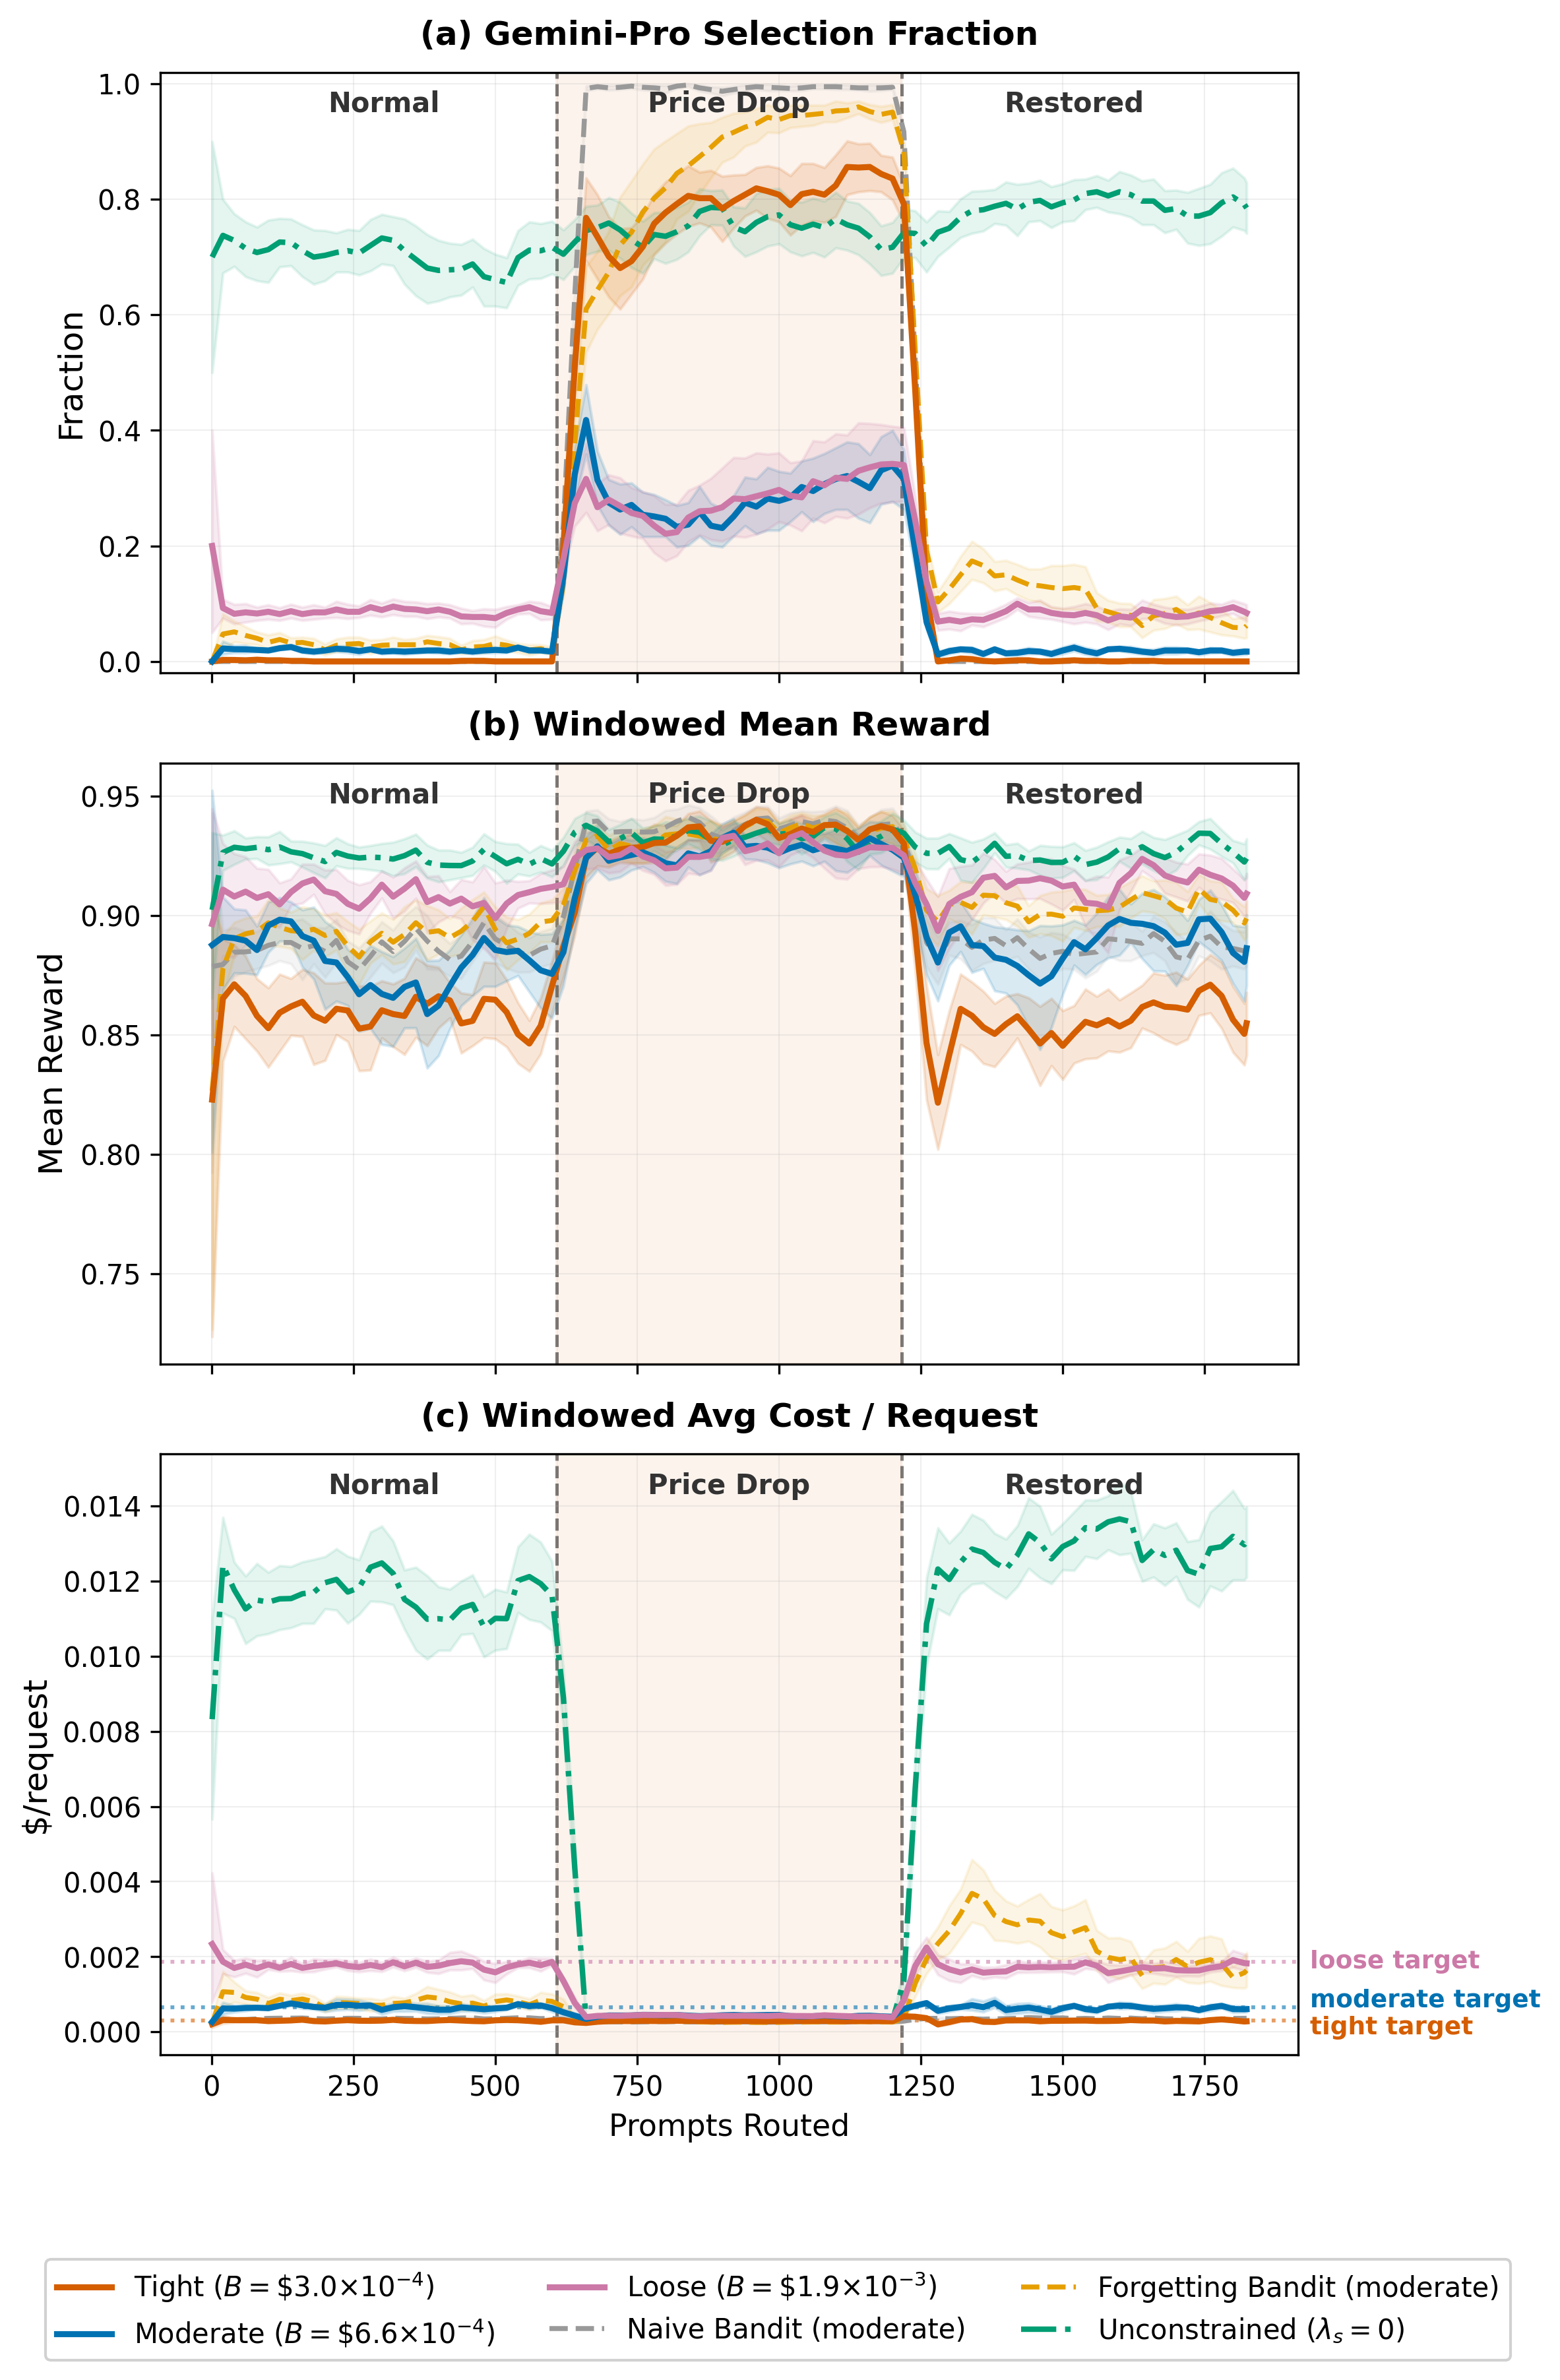
\includegraphics[width=\columnwidth]{../experiments/02_budget_plus_drift/results/adaptation_dynamics.png}
\caption{Adaptation dynamics under cost drift ($K{=}3$, 20~seeds, 95\% bootstrap CI). Normal pricing $\to$ Gemini price drop at prompt~$\cfPhaseN$ $\to$ price restored at prompt~$2{\times}\cfPhaseN$. \textbf{(a)}~Gemini-Pro selection fraction: all budget tiers surge toward Gemini during the price drop, then revert when pricing is restored. \textbf{(b)}~Windowed mean reward: all conditions improve during Phase~2 as Gemini becomes budget-accessible. \textbf{(c)}~Windowed average cost per request (dotted = budget ceilings): ParetoBandit tracks the ceiling in all three phases; the Forgetting Bandit overshoots from Phase~1 onward.
}
\label{fig:adaptation_dynamics}
\end{figure}

\noindent\textbf{Results (Figure~\ref{fig:catastrophic_failure}).}  ParetoBandit detects the quality drop purely through the reward signal, reducing Mistral allocation from $\cfParetoBanditModMistralPhaseOne$\% to $\cfParetoBanditModMistralPhaseTwo$\% in Phase~2 at moderate budget.  In Phase~3, geometric forgetting down-weights the corrupted estimates and staleness-driven exploration begins re-exploring Mistral, raising allocation to $\cfParetoBanditModMistralPhaseThree$\% and recovering Phase~3 reward to $\cfParetoBanditModPhaseThreeReward$\,[$\cfParetoBanditModPhaseThreeRewardCILo$, $\cfParetoBanditModPhaseThreeRewardCIHi$] (vs.\ Phase~1 $\cfParetoBanditModPhaseOneReward$\,[$\cfParetoBanditModPhaseOneRewardCILo$, $\cfParetoBanditModPhaseOneRewardCIHi$], recovery ratio $\cfParetoBanditModRecoveryMean$\,[$\cfParetoBanditModRecoveryCILo$, $\cfParetoBanditModRecoveryCIHi$]).  Budget compliance holds throughout ($\cfParetoBanditLoosePhaseOneRatio$\,[$\cfParetoBanditLoosePhaseOneRatioCILo$, $\cfParetoBanditLoosePhaseOneRatioCIHi$] to $\cfParetoBanditTightPhaseOneRatio$\,[$\cfParetoBanditTightPhaseOneRatioCILo$, $\cfParetoBanditTightPhaseOneRatioCIHi$] across all nine phase--budget cells).  The unconstrained baseline is unaffected (Phase~2 reward $\cfUncPhaseTwoReward$\,[$\cfUncPhaseTwoRewardCILo$, $\cfUncPhaseTwoRewardCIHi$] vs.\ Phase~1 $\cfUncPhaseOneReward$\,[$\cfUncPhaseOneRewardCILo$, $\cfUncPhaseOneRewardCIHi$]) but incurs a $\cfUncCostSpikePct$\% cost increase from over-allocating to Gemini.  This ${\sim}\ppCfDegPct$\% degradation lies within the system's recovery envelope; Appendix~\ref{appendix:recovery_limit} characterises the threshold beyond which recovery requires an extended horizon.
\begin{figure}[!t]
\centering
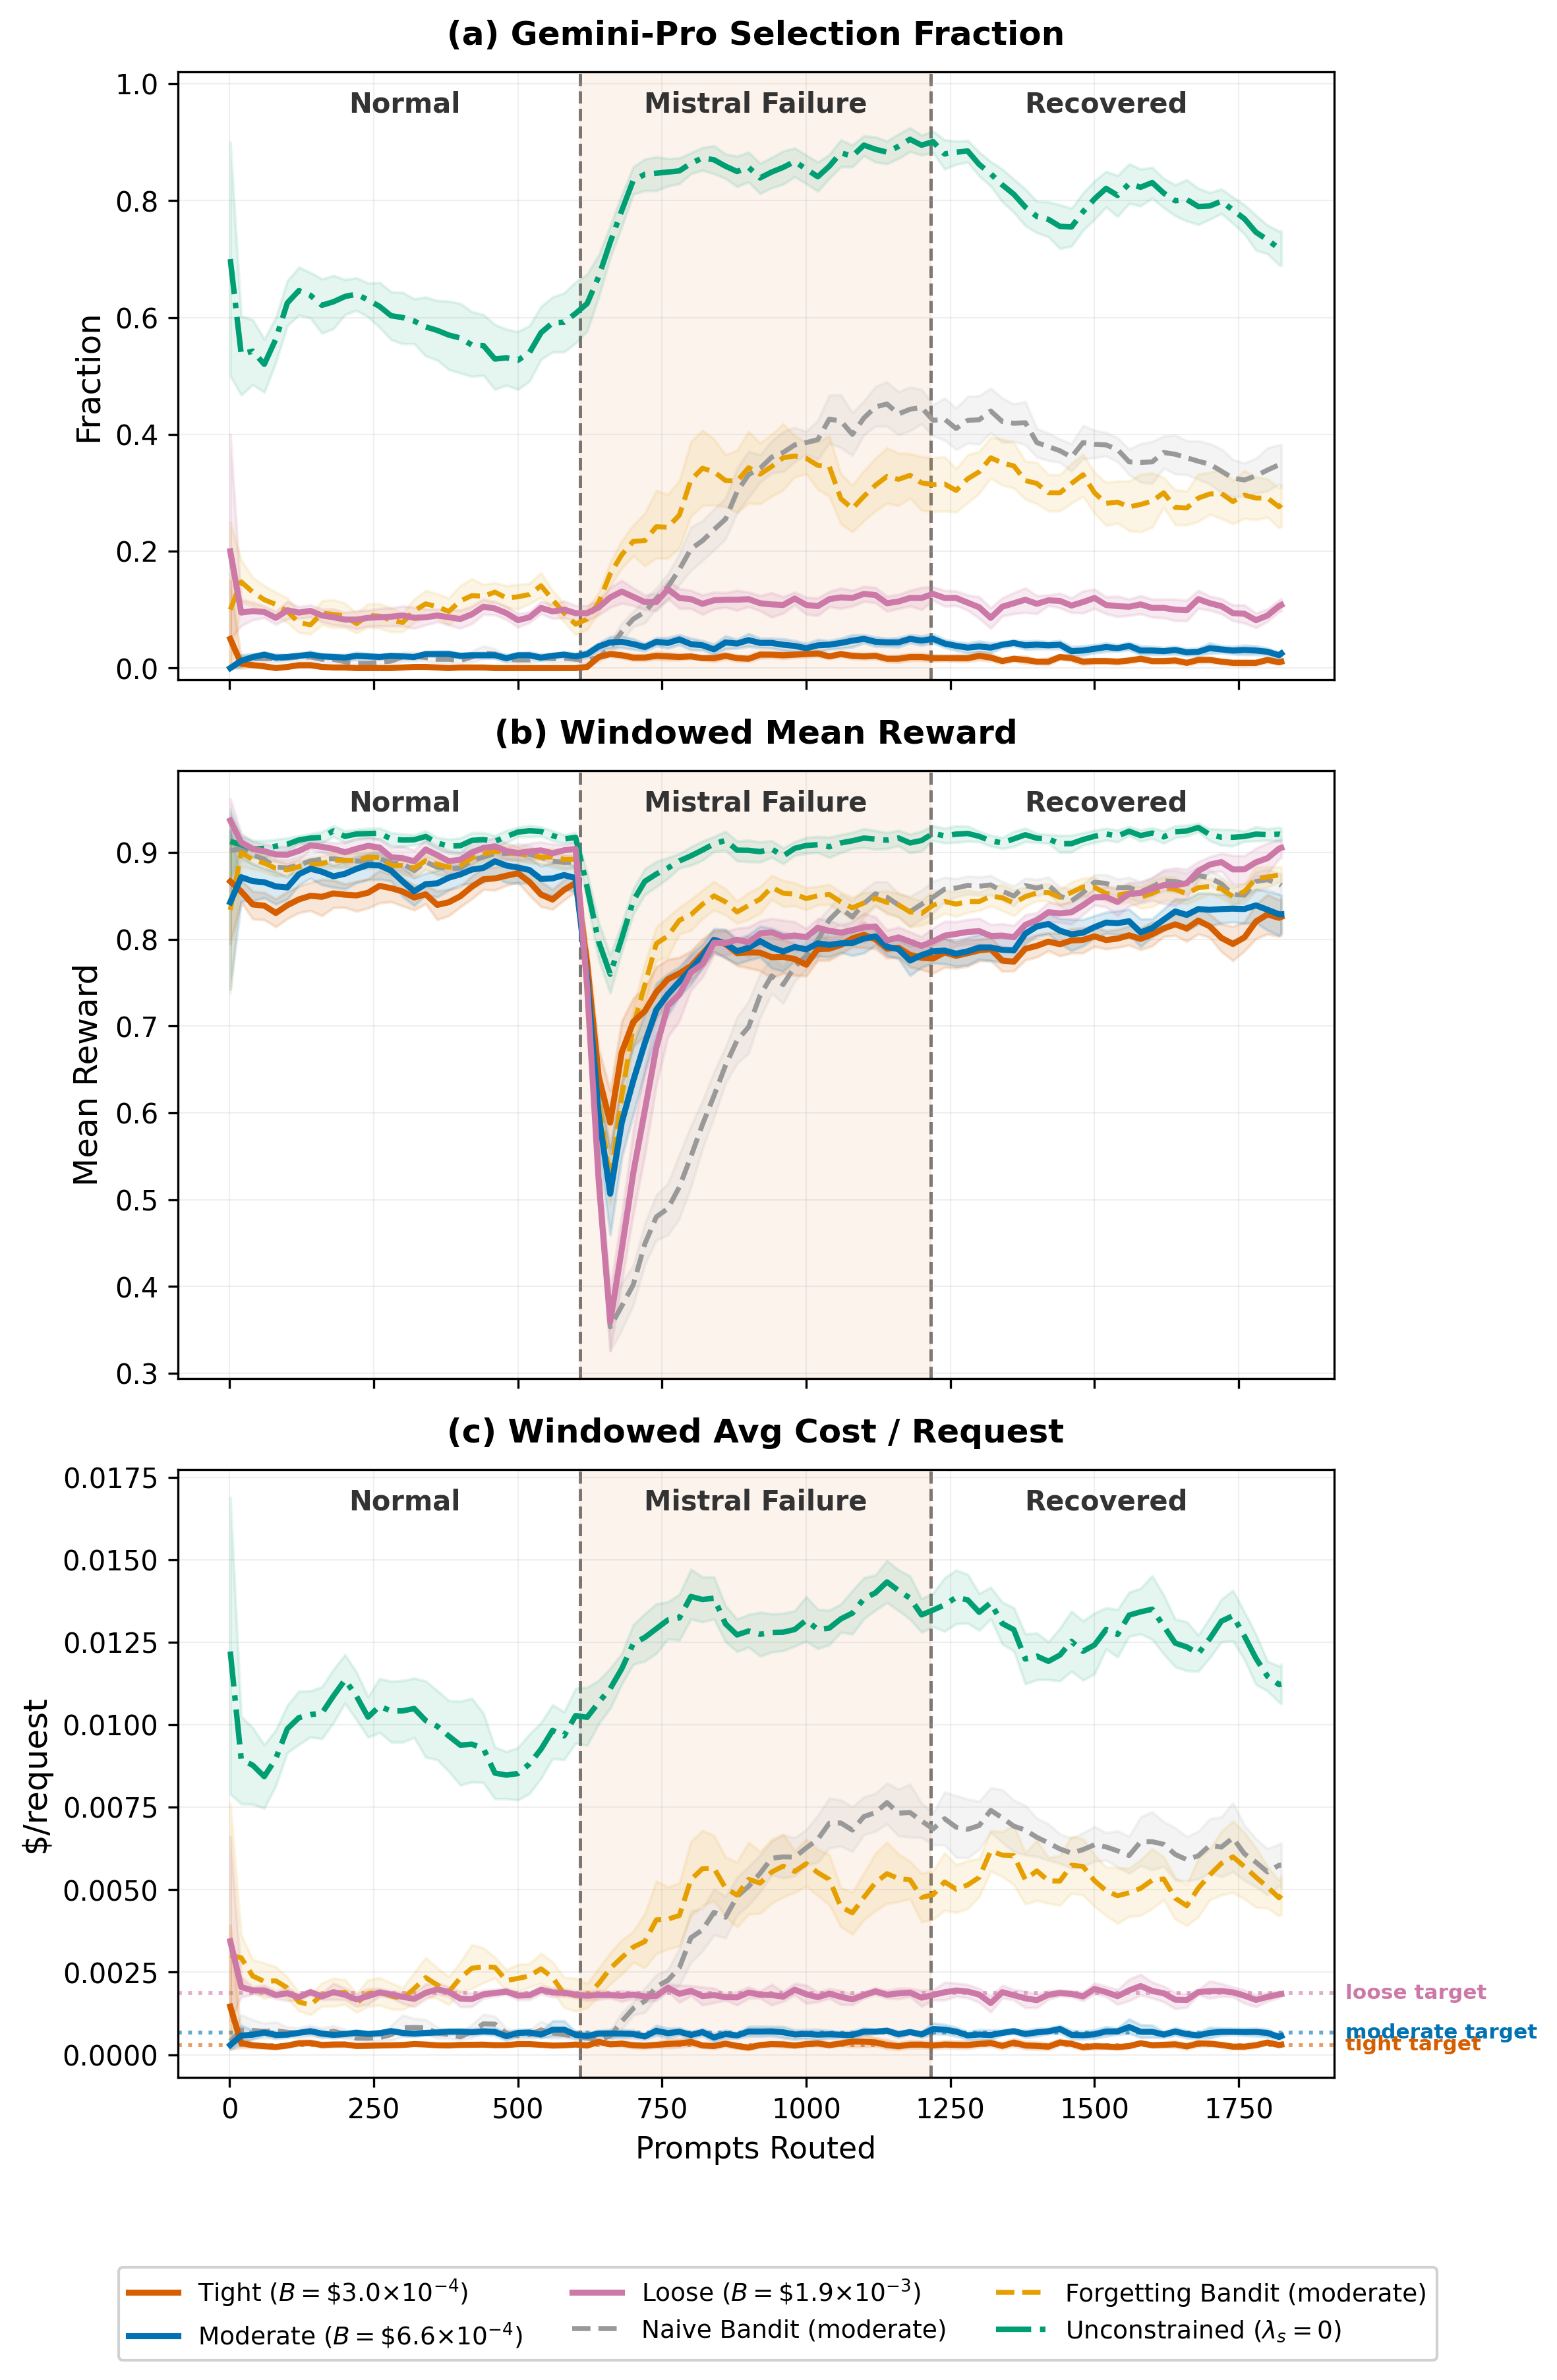
\includegraphics[width=\columnwidth]{../experiments/03_catastrophic_failure/results/catastrophic_failure_dynamics.png}
\caption{Quality degradation dynamics (Normal $\to$ Mistral degradation at prompt~$\cfPhaseN$ $\to$ recovered at prompt~$2{\times}\cfPhaseN$; 20~seeds, 95\% bootstrap CI).  \textbf{(a)}~Gemini-Pro selection fraction: constrained budgets shift modestly; the unconstrained baseline shifts ${\sim}17$\,pp toward Gemini.  \textbf{(b)}~Windowed mean reward: all adaptive conditions detect the quality drop; the loose budget and unconstrained baseline recover fully in Phase~3, while tighter budgets are still converging at the horizon limit (Appendix~\ref{appendix:recovery_limit}).  \textbf{(c)}~Cost per request (dotted = budget ceilings): ParetoBandit tracks the ceiling throughout; cost stability confirms the degradation is invisible to the cost signal.
}
\label{fig:catastrophic_failure}
\vspace{-10pt}
\end{figure}

\subsection{Cold-Start Model Onboarding}
\label{sec:eval_onboarding}

After Phase~1 learning on the $K{=}3$ portfolio, Gemini-2.5-Flash is added as a fourth arm via \texttt{register\_model()} with no warmup priors. Figure~\ref{fig:model_onboarding} shows Flash adoption across three scenario--budget combinations. In the Good \& Cheap scenario (Figure~\ref{fig:model_onboarding}a), all 80 trials (20~seeds $\times$ 4~budget tiers) achieve sustained adoption within ${\sim}\ppAdoptionSteps$ steps. Budget determines the equilibrium share, not whether adoption occurs: loose budgets settle at ${\sim}\moGoodCheapPBLooseFlashFinalPct$\%\,[$\moGoodCheapPBLooseFlashFinalPctCILo$, $\moGoodCheapPBLooseFlashFinalPctCIHi$] Flash share while tight budgets plateau at ${\sim}\moGoodCheapPBTightFlashFinalPct$\%\,[$\moGoodCheapPBTightFlashFinalPctCILo$, $\moGoodCheapPBTightFlashFinalPctCIHi$]. The BudgetPacer maintains compliance throughout the $K{=}3 \to K{=}4$ transition without reconfiguration (Figure~\ref{fig:model_onboarding_cost}). Crucially, the bandit discriminates rather than blindly adopting: expensive models are budget-gated (Figure~\ref{fig:model_onboarding}b) and bad models are rejected after a bounded burn-in (Figure~\ref{fig:model_onboarding}c).

\begin{figure*}[!t]
\centering
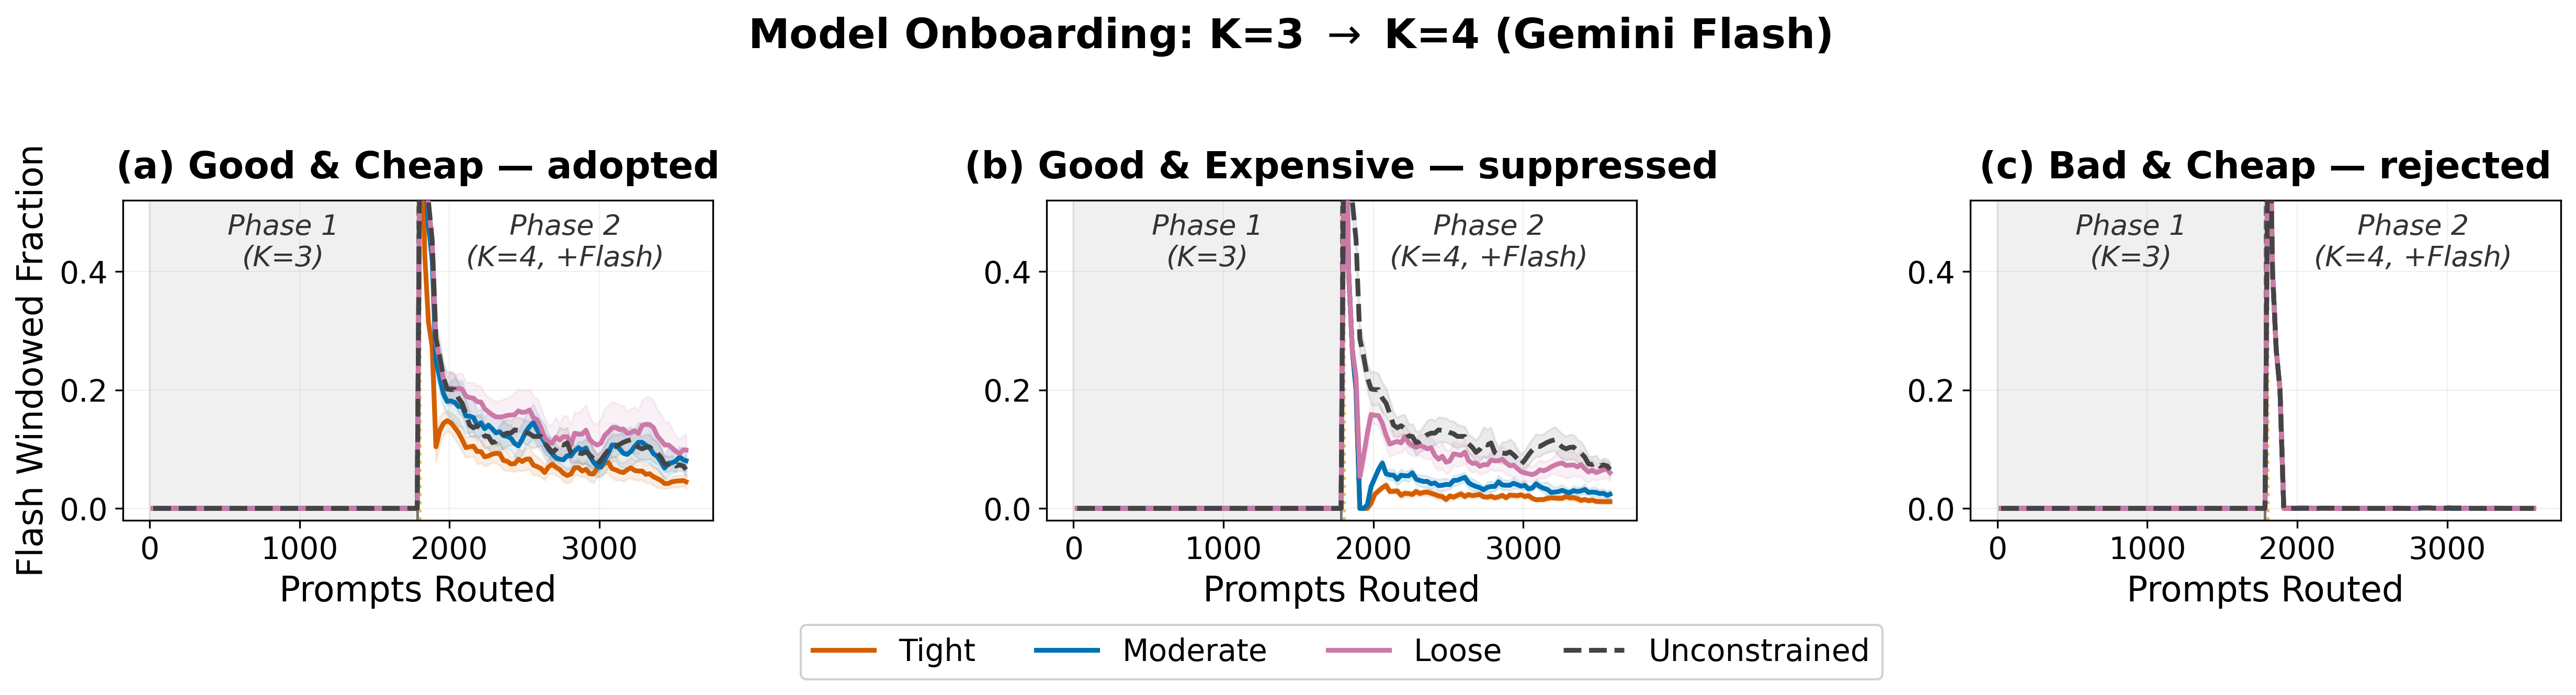
\includegraphics[width=\textwidth]{../experiments/04_model_onboarding/results/model_onboarding.png}
\caption{Model onboarding ($K{=}3 \to K{=}4$; 20~seeds, 95\% bootstrap CI). Flash windowed selection fraction across four budget levels after cold-start addition. \textbf{(a)}~Good \& cheap: Flash is adopted at all budgets. \textbf{(b)}~Good \& expensive: the BudgetPacer suppresses Flash under tight budgets. \textbf{(c)}~Bad \& cheap: the bandit correctly rejects Flash in every seed.
}
\label{fig:model_onboarding}
\vspace{-4pt}
\end{figure*}

The trade-off relative to offline characterisation is that ${\sim}1$\% of Phase~2 requests serve as online exploration, but adoption is automatically budget-gated and requires no paired preference data.

\begin{figure}[!t]
\centering
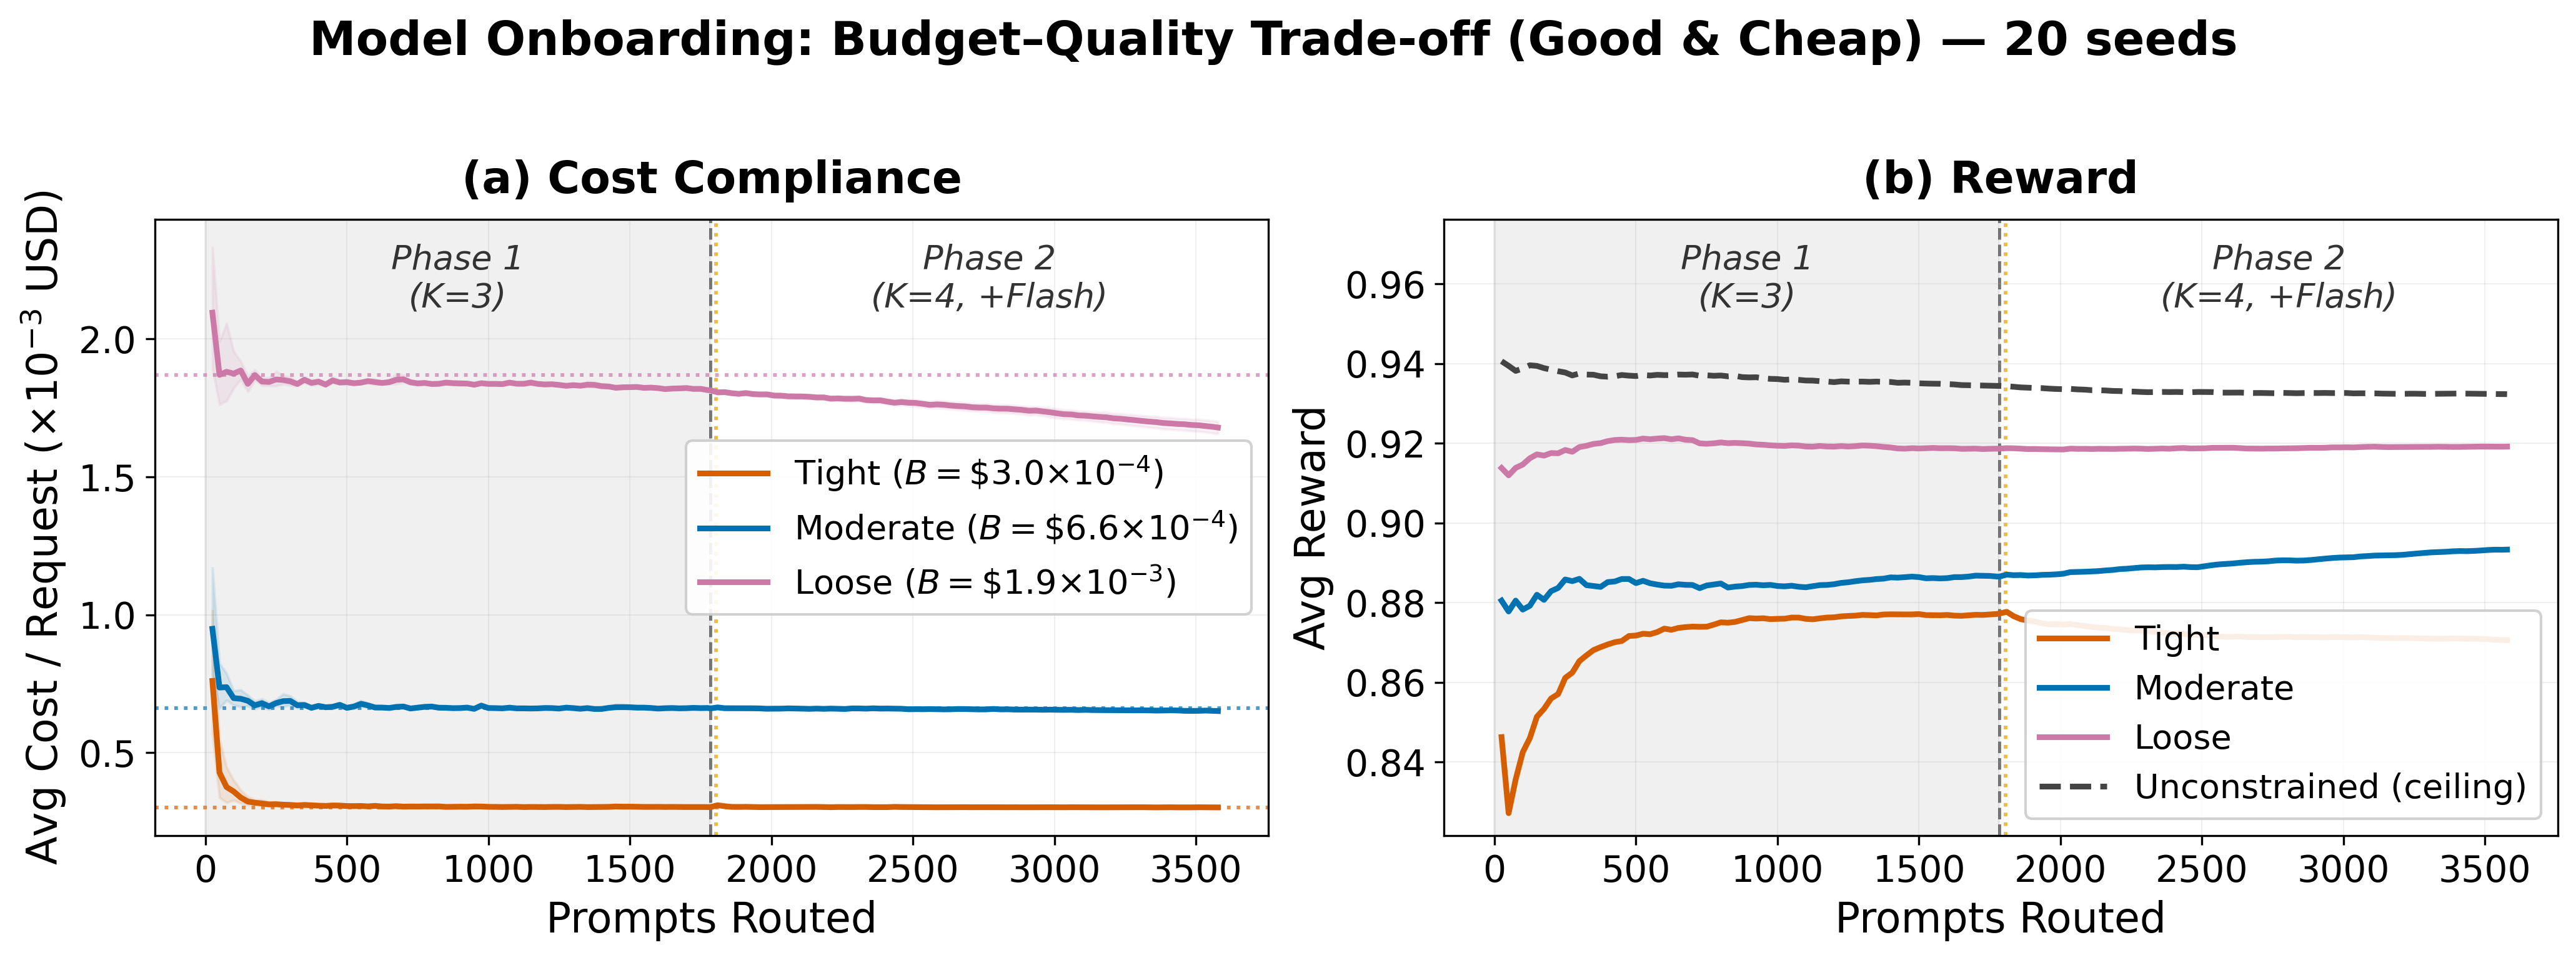
\includegraphics[width=0.6\columnwidth]{../experiments/04_model_onboarding/results/model_onboarding_cost.png}
\caption{Budget--quality trade-off during model onboarding (Good \& Cheap; 20~seeds, 95\% bootstrap CI).
(a)~Running average cost per request (dotted = targets). Tight and moderate track their ceilings to within 1\% throughout the $K{=}3 \to K{=}4$ transition; the loose tier settles ${\sim}6$\% below target due to complementary slackness ($\lambda_t \approx 0.06$ vs.\ $0.41$ at tight).
(b)~Cumulative average reward. Tight budget dips ${\sim}1$\% at the Phase~2 boundary (cost of 20 forced-exploration pulls). Moderate reward rises $1$\% as Flash fills a quality niche previously inaccessible at that tier. Loose and unconstrained rewards confirm the budget constraint is non-binding.
}
\label{fig:model_onboarding_cost}
\vspace{-6pt}
\end{figure}
